\section{Presentation Logic Layer}
\graphicspath{ {./HW_1/images/} }
%What pages will be present in your project? briefly indicate how your web site will be organized

The website will be divided into the following pages:
\begin{itemize}
    \item Homepage: contains the main area with the sections AboutUs and ContactUs. Allows users to login or register to the system through LOGIN and REGISTER buttons, respectively. Developed via jsp.
    \item Login page: allows the users login to the LMS. Developed via jsp.
    \item Registration page: allows students to register in the LMS.
    \item Administration page: allows to administrate users’ accounts. Written in HTML.
    \item Teacher page: allows users to search for maintenance events. written in HTML with the
support of javascript.
    \item List students page: allows to insert a new maintenance event. Written in HTML.
    \item List teachers page: allows to upload a file containing the measurements. Written in HTML.
    \item Teacher dashboard page: allows to redirect users toward pages handling specific resources. Written in HTML.
    \item Available teachers page:
    \item About Us page:
    \item Contact Us page:
    \item Post material page:
    \item RegisterWireframePage:
    \item RequestCoursePage:
    \item StudentDashboardPage:
    \item SendQueryTeacherPage:
    \item SubjectAreaPage:
    \item 2 pages each to handle insertion and update of parks, rides and models. Written in HTML.
    
    \item A support page which displays messages upon completion of specific tasks, such as the removal or update
of resources.
\end{itemize}

\subsection{Login Form}

%For the main pages put a mockup and describe it in detail.

\subsection{Homepage}
The homepage contains the LOGIN button for the users who has already registered and using the system and the Register button for new users. Pressing the REGISTER button the user will go to the student registration page. The left-side area of the homepage will contain the information sections as About Us and Contact Us. There will be the description of the TORE project, contact links for our social media pages and the contact form for sending us messages.\\ 

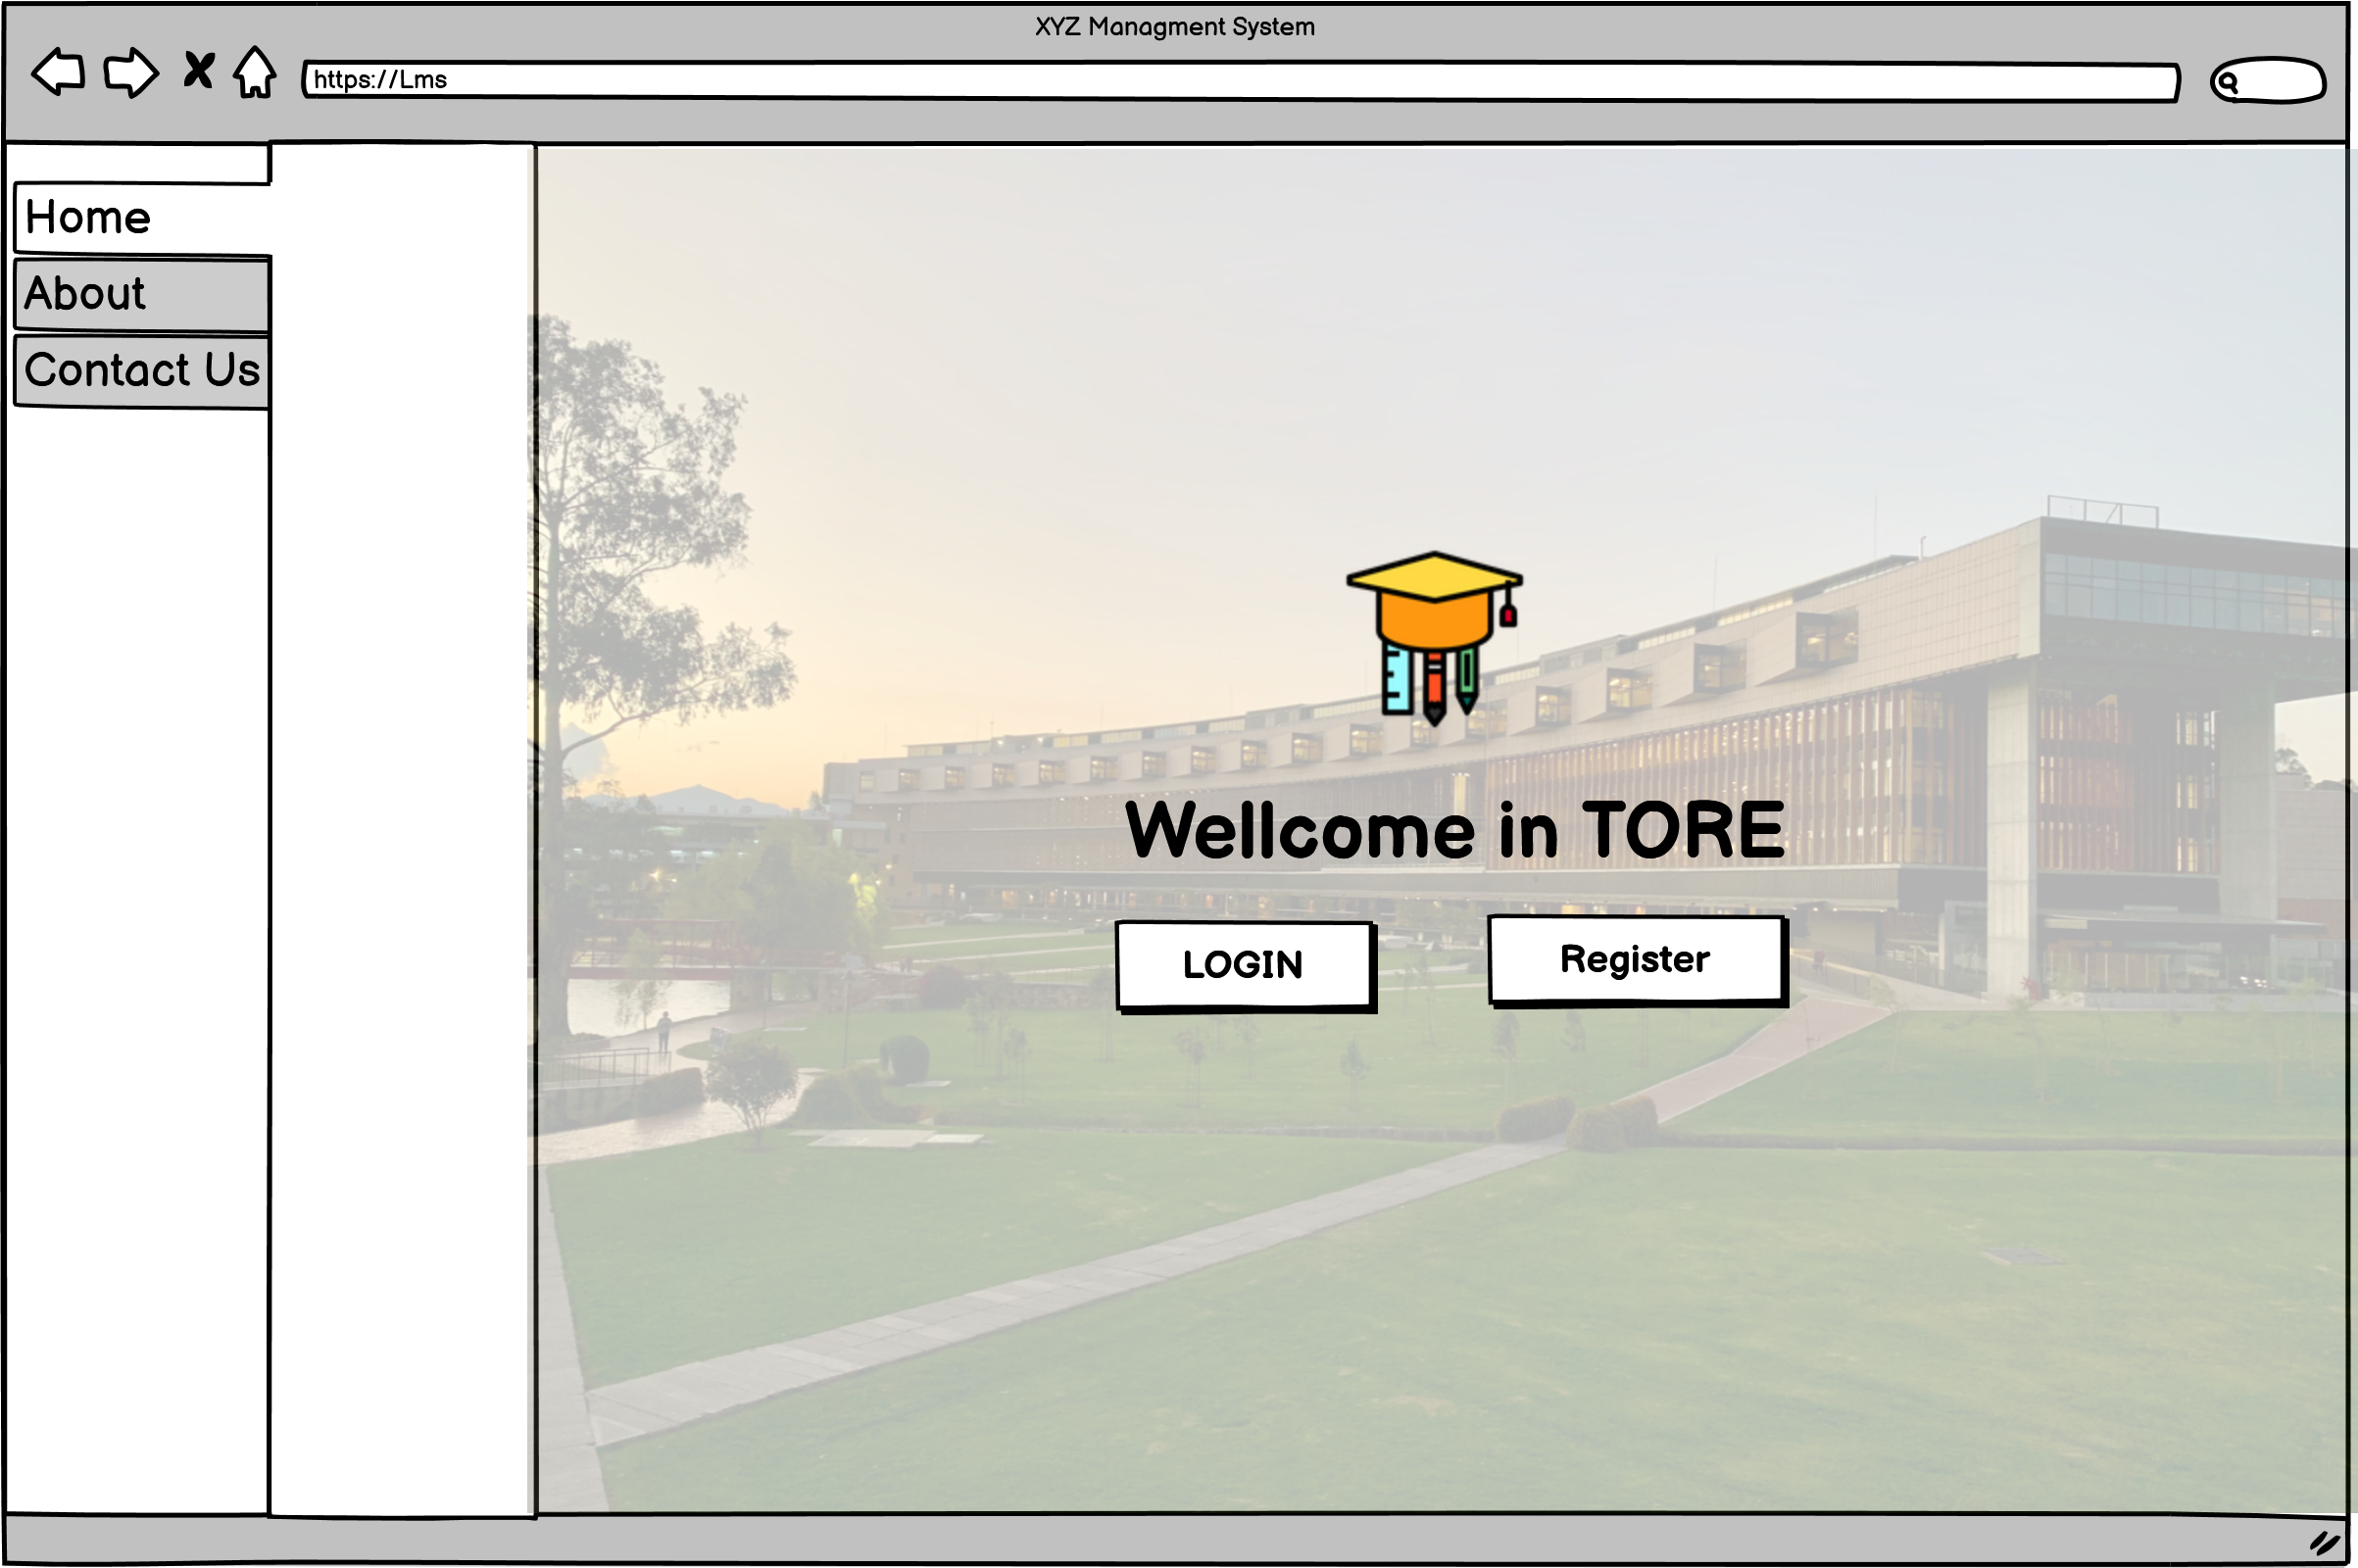
\includegraphics[width=\columnwidth]{images/HomePage.png}
\newpage
The about us page contains the information about the TORE system and all useful links to contact with us.\\

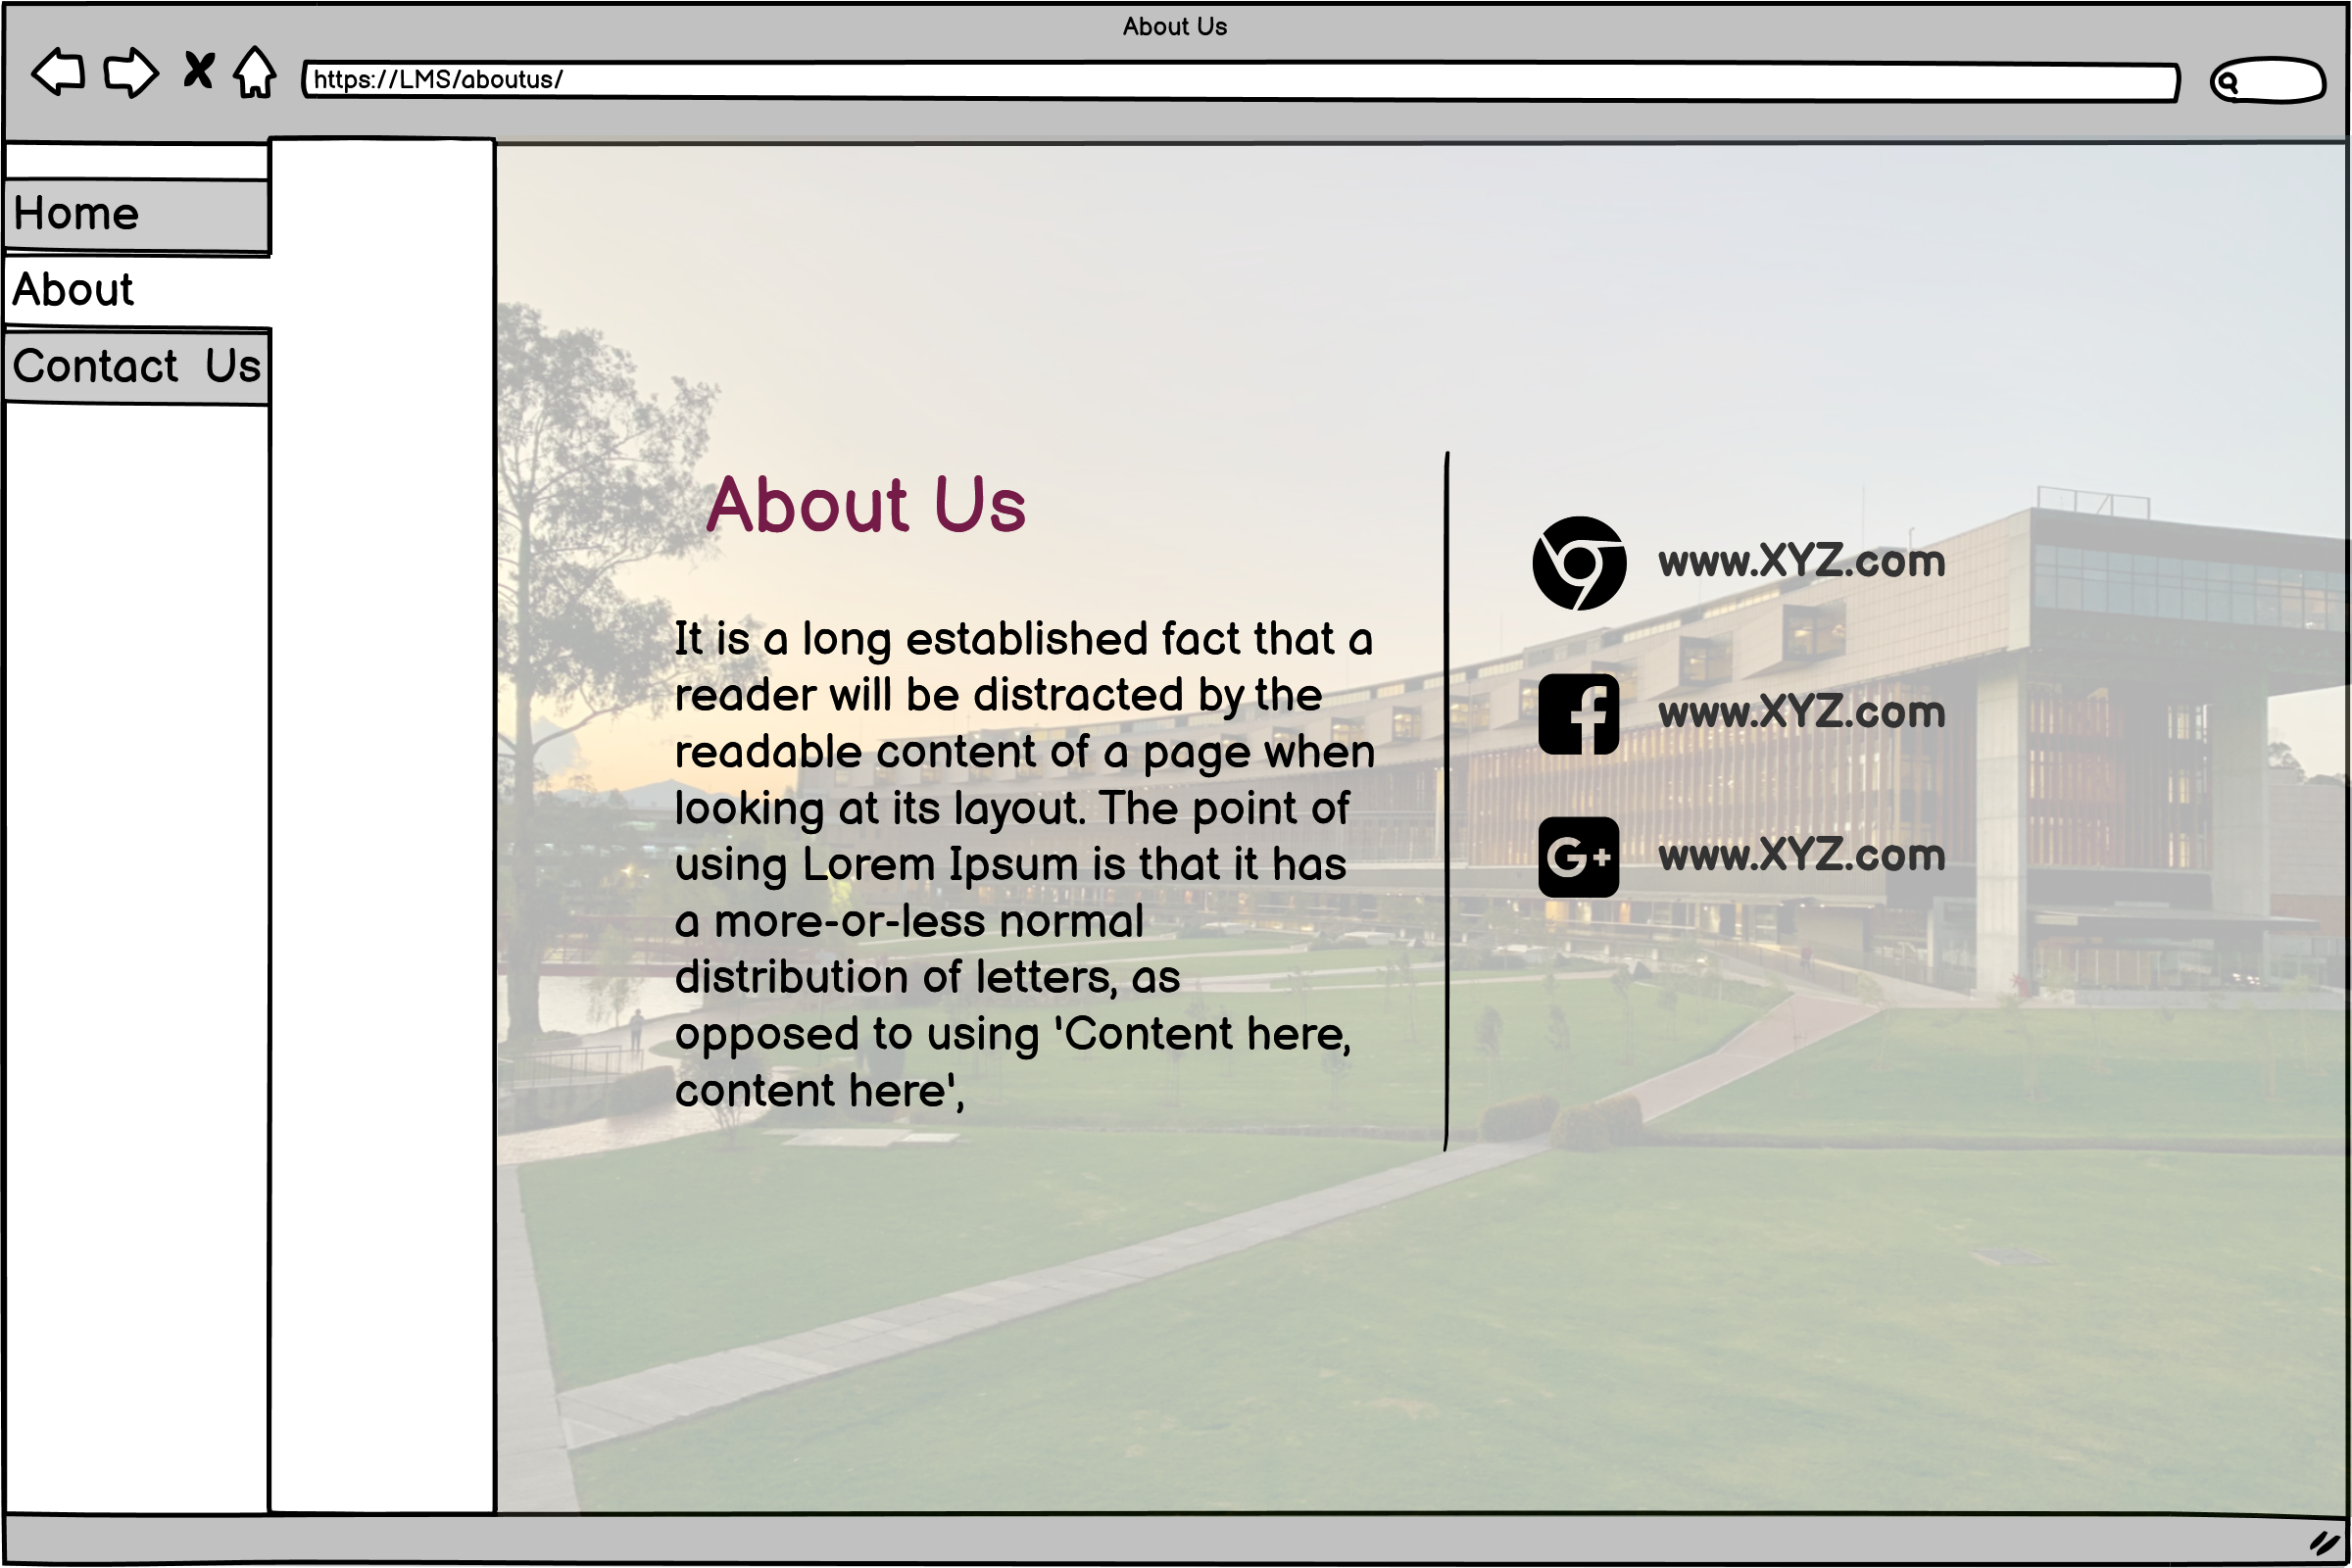
\includegraphics[width=\columnwidth]{images/New Wireframe 2.png}
\newpage
The contact us page contains a form for manual filling in the name of the user, the subject of the message and the description of the topic. By clicking the “Submit” button, the message is send.\\

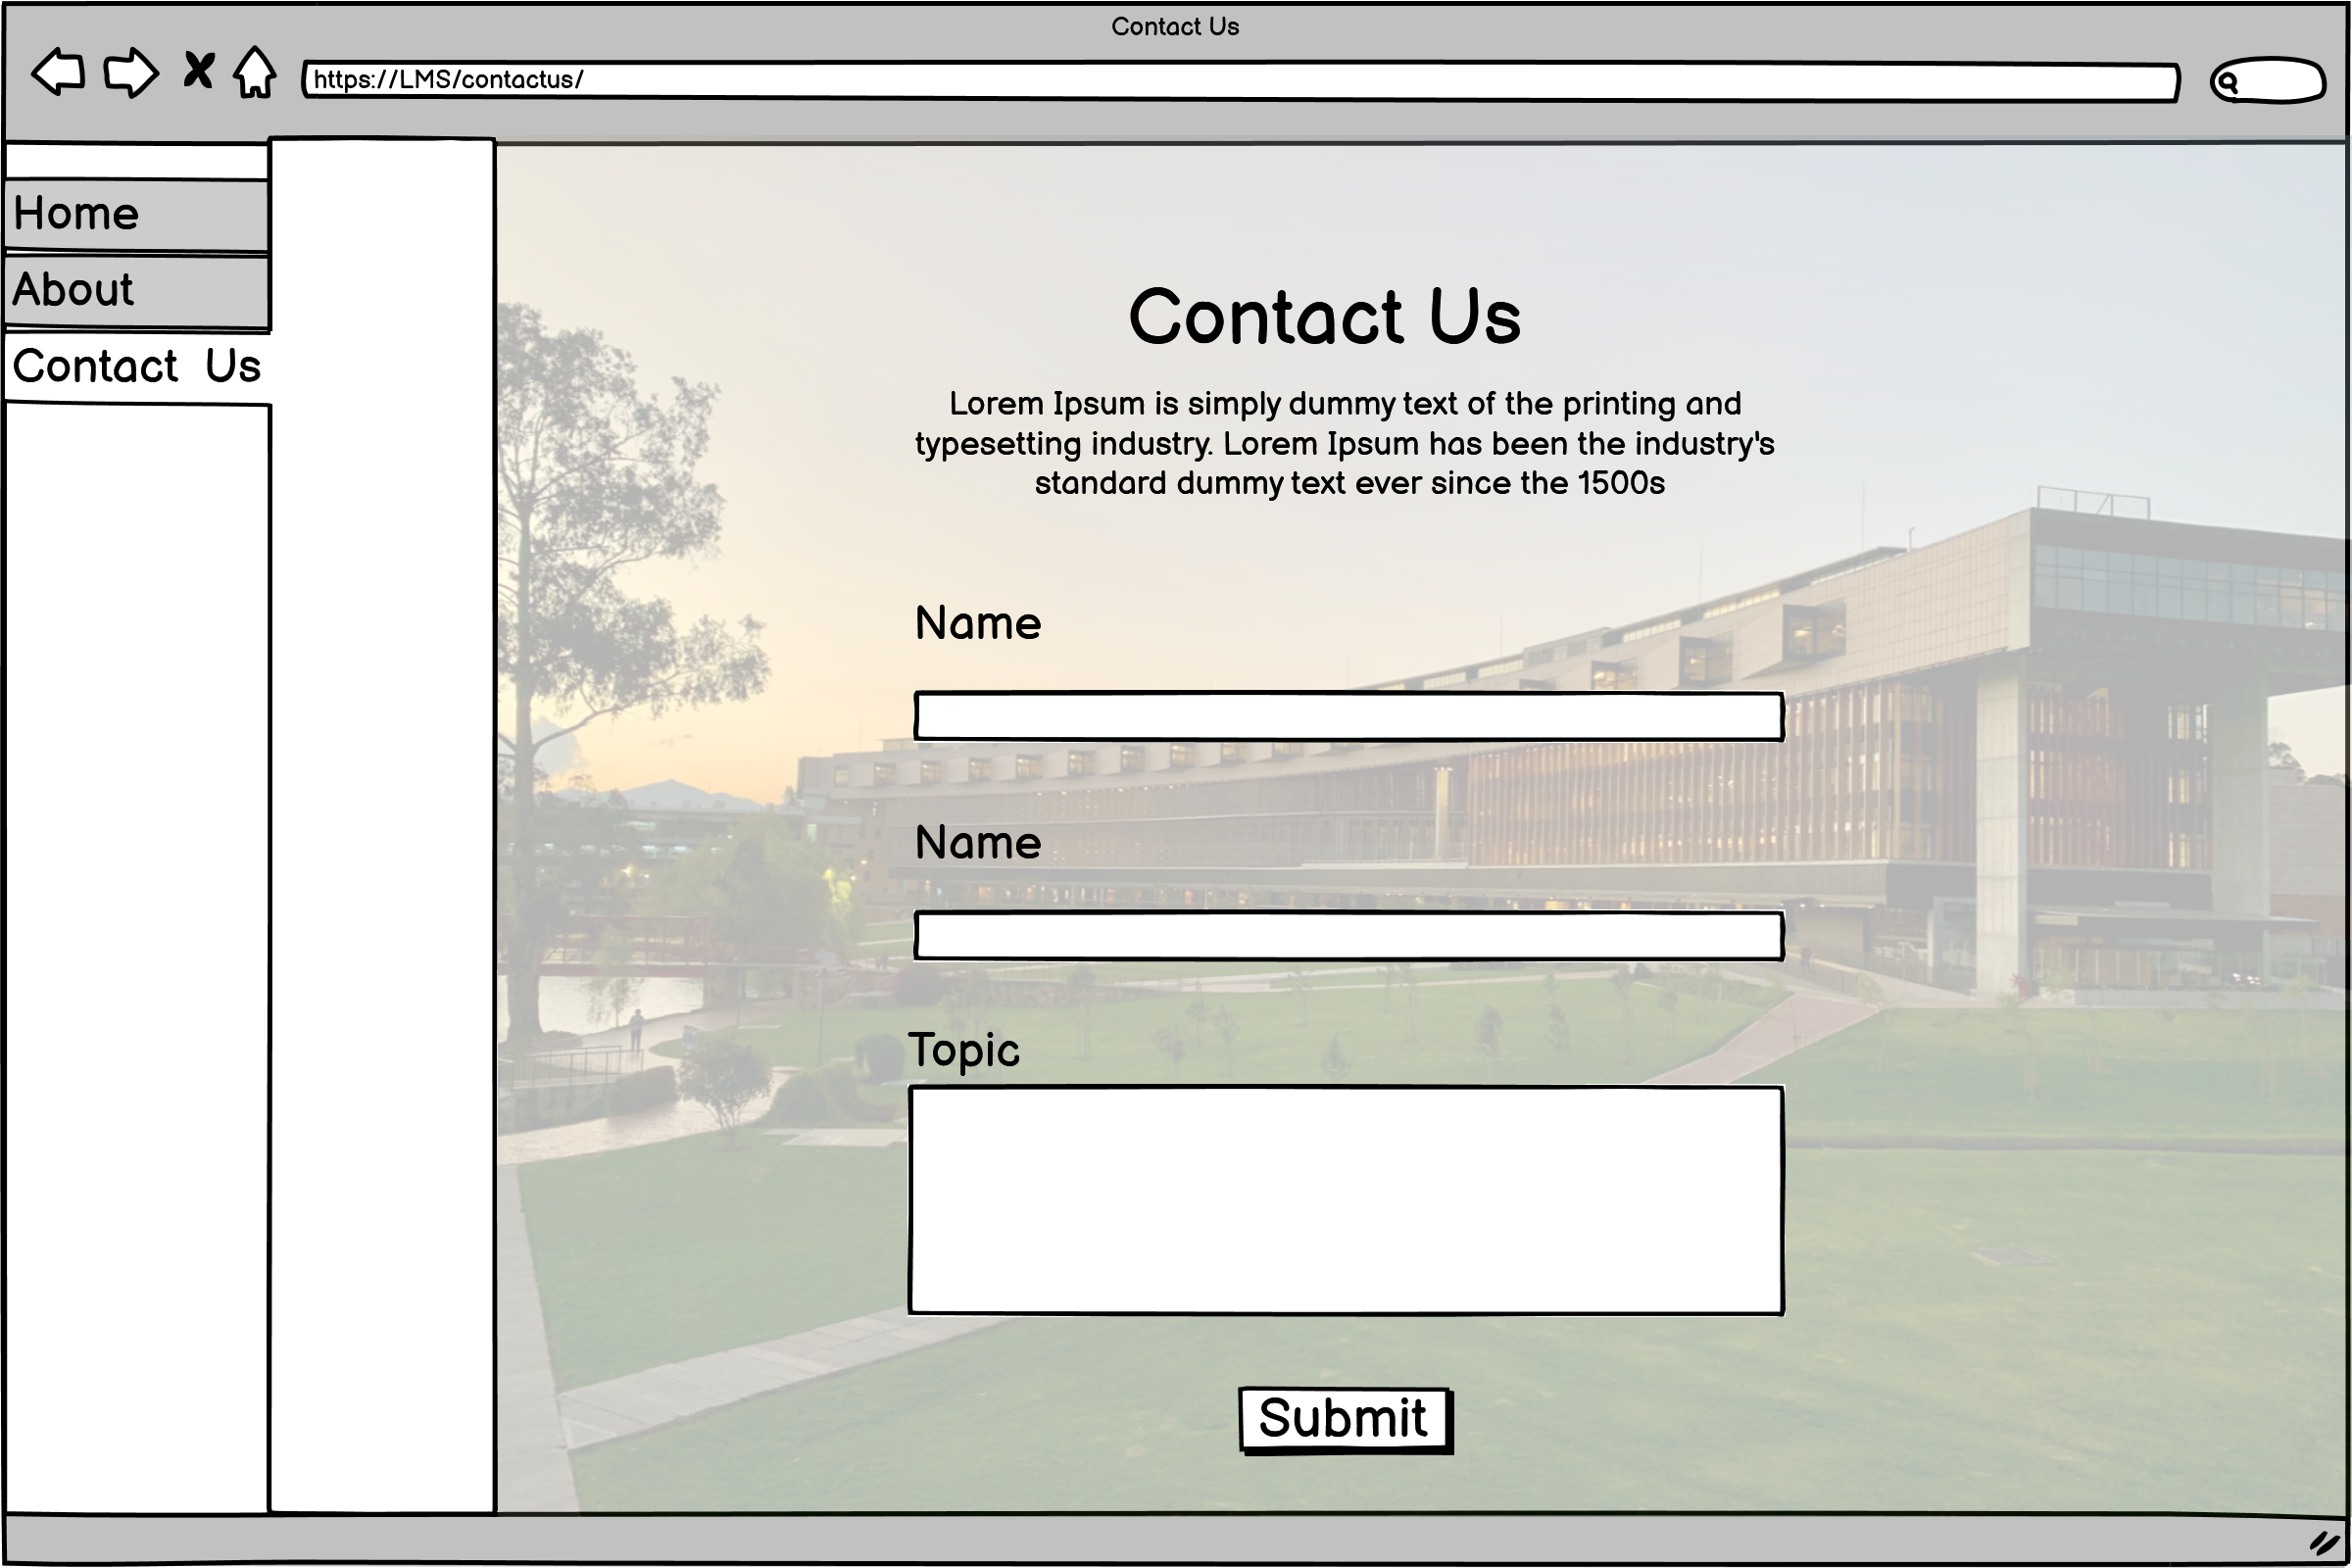
\includegraphics[width=\columnwidth]{images/New Wireframe 3.png}
\newpage
\subsection{Login Page}
  
The login page contains the form used to having an access to users own page inside the system. There are two input fields for e-mail address and the password, respectively. The user can select his/her status at the category field as teacher, student or admin. By pressing the LOGIN button the user will go to the personal page with all the information concerning his/her courses that are in progress or have already been finished.\\

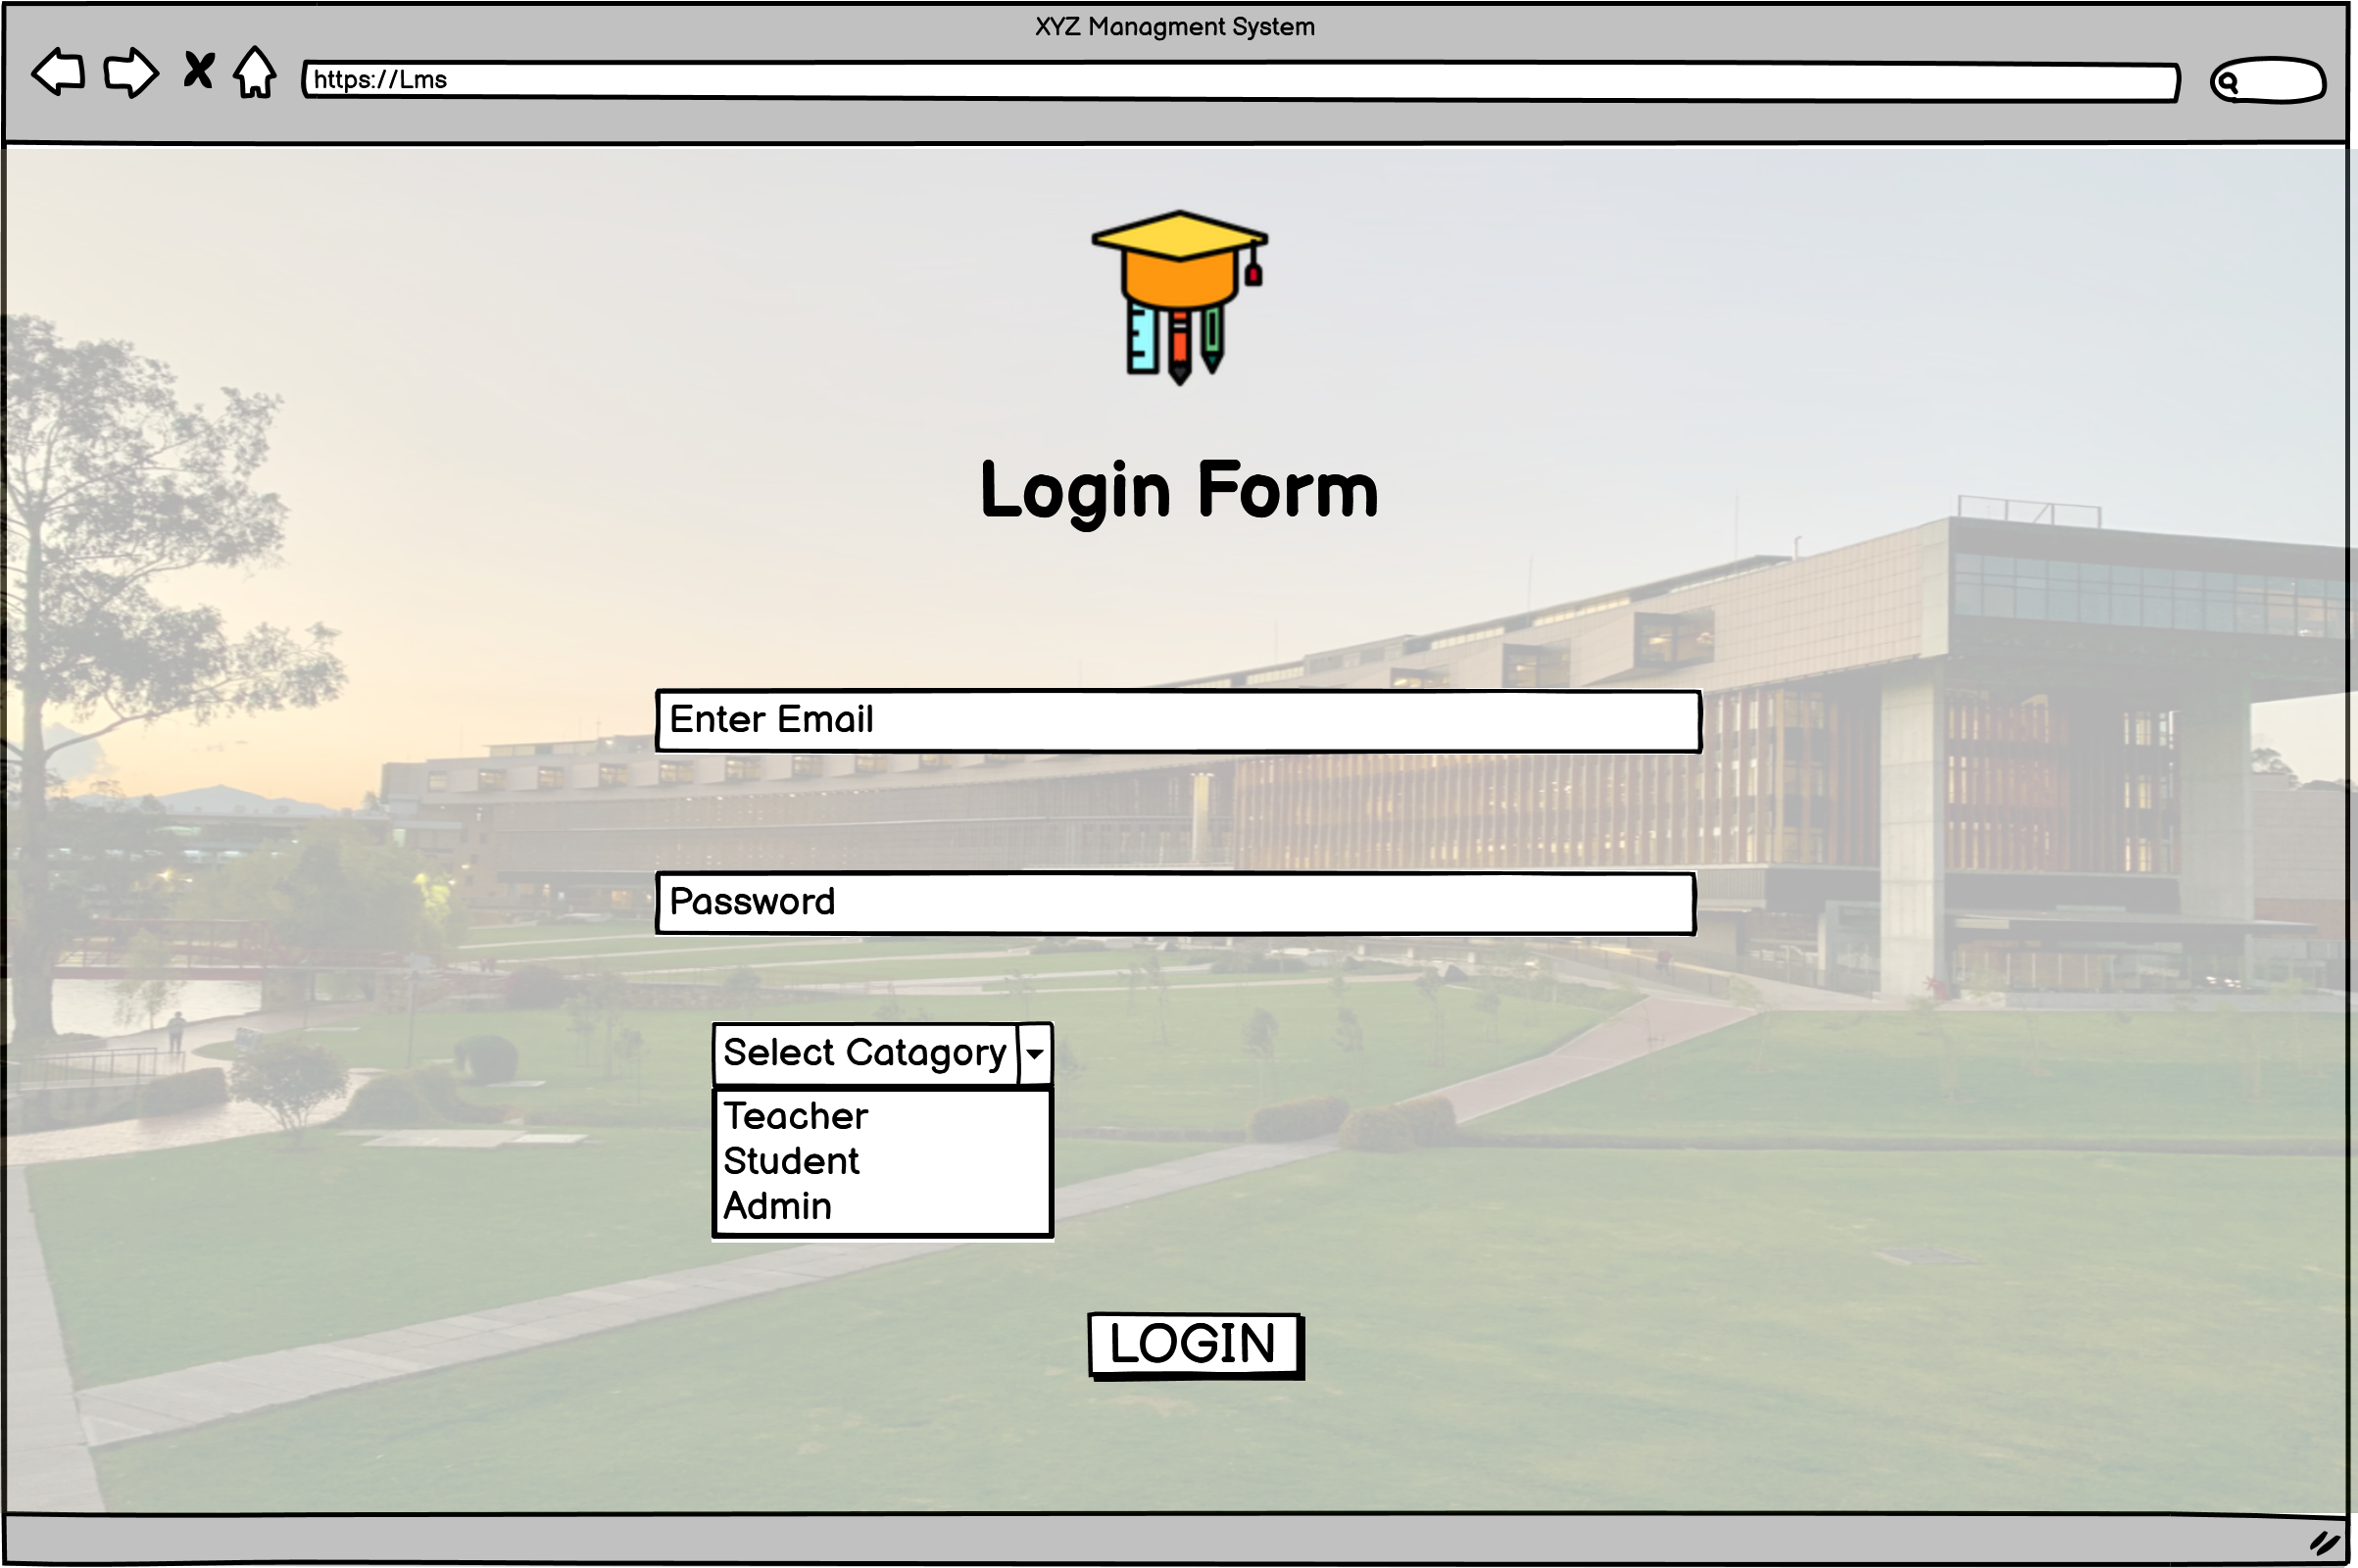
\includegraphics[width=\columnwidth]{images/LoginForm.png}
\subsection{Student registration page}
  
The registration page contains a form for manual filling in the name, e-mail, address and password. The Gender field gives the option to choose between three variants and at the Birth Date field the date can be selected from the database. After the form is filled in the user submitting it and sending the register request to admin by clicking the Register button. Getting the register request from user the admin gives the access to the portal or decline it. If the register request is approved for the user he/she will have the ability to login to the portal.  

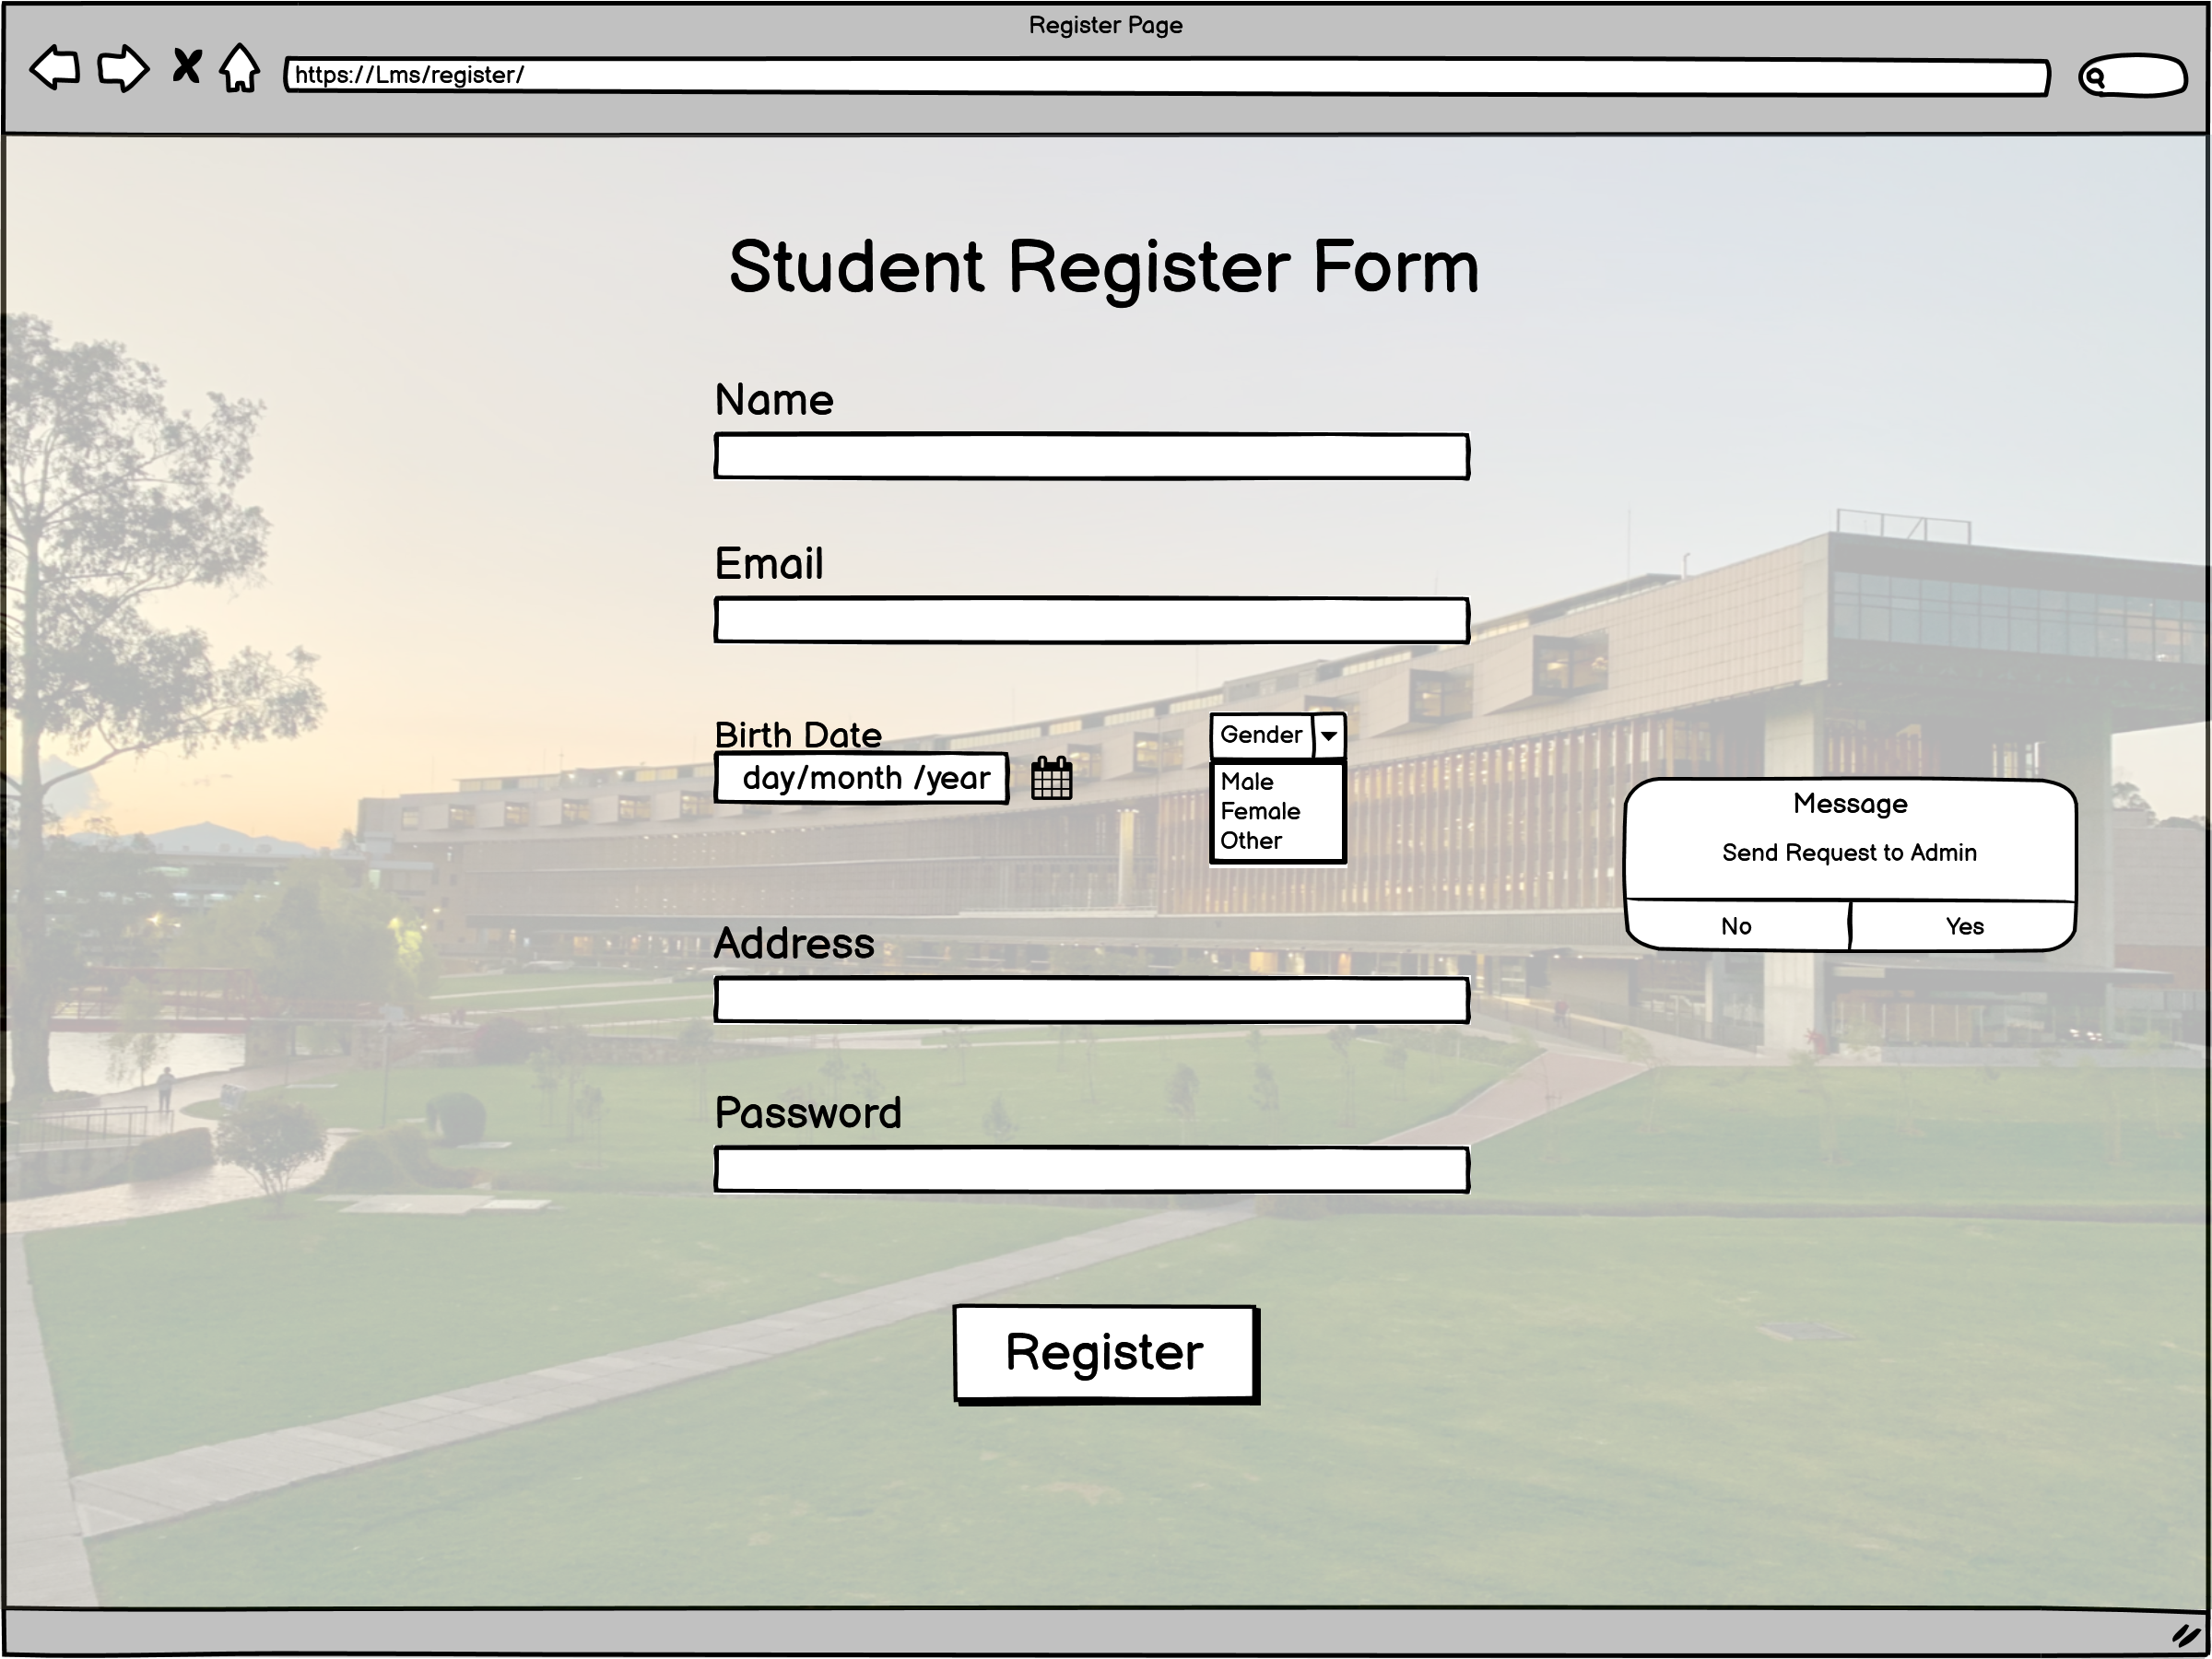
\includegraphics[width=\columnwidth]{images/StudentRegisterForm.png}
\subsection{Admin Page}
The admin page is divided into three sections: “search”, “user details” and “update user details”. Upon
entering the page, only the “search” section will be filled.\\

The admin page allows to search for users via email. The selector is filled automatically with the emails
of all the registered users. Once the email of the user has been specified, by clicking on the “Search”
button, the two following sections (“user details” and “update user details”) are automatically filled with
the information on the users. In particular, in the section “user details” is reported a table with the user
email, first name, last name and role.\\ 

The section “update user details” contains a form, automatically filled with the data on the searched
user. The admin can update such data. They can then click on either the button “update” which
updates the user details, or the button “delete” which deletes the user from the database, revoking
their possibility to login and therefore to access reserved areas of the website.

\includegraphics[width=\columnwidth]{images/amupark_admin.png}
\subsection{Builder Page}
The general builder page is organized into folders. Each folder corresponds to a specific entity in the dataset, among those that can be managed by the builders. In particular, we have a folder for the parks, one for the rides and one for the models. By clicking on each folder, the user is presented with the interface to interact with the requested resource. In particular, there is a link that allows the user to reach the page for inserting a new resource and a selector that allows the user to select a specific resource based on its unique identifier and reach the page to edit it.

\includegraphics[width=\columnwidth]{images/amupark_builder.png}
\subsection{Search Maintenance Page}
The “search maintenance page” contains a form used to filter out maintenance events. The user can select the ride to which the searched maintenance events refer to. They can filter events with two checkboxes to select either only events planned, not planned or both.\\

There are also two date input fields, they can be used to filter maintenance events in order to select only maintenance events occurring between two specific dates.


\includegraphics[width=\columnwidth]{images/amupark_maintenance.png}
\subsection{Insert Ride Page}
The Insert Rides Page contains the form necessary to insert a new ride.\\

There is a static and a dynamic part of the page. In the static part, it is possible to insert the description of the ride, the park it is going to be deployed in and its model. Both the park input and the model input are going to be filled automatically, based on the data available in the database.\\

Dynamic aspects of the page regard the possibility of adding (and removing) on the fly additional devices that are mounted on the ride. By clicking on a “+” button, a new device form will be inserted in the device form area. There is also a “-” button, which will allow the user to remove devices. Note that, each device form will have its own “-” button. This way, the user can remove specific devices, without the need for additional effort that might stem from the removal of the last inserted device.\\

Upon completion, if the insertion ended correctly, the user is redirected to the homepage.

\includegraphics[width=\columnwidth]{images/amupark_insertnew.png}
%\input{sections/PLL/TeacherDashboardPage.tex}
%\input{sections/PLL/AvailableTeachersPage.tex}
%\input{sections/PLL/AboutUsPage.tex}
%\input{sections/PLL/ContactUsPage.tex}
%\input{sections/PLL/PostMaterialPage.tex}
%\input{sections/PLL/RegisterWireframePage.tex}
%\input{sections/PLL/RequestCoursePage.tex}
%\input{sections/PLL/StudentDashboardPage.tex}
%\input{sections/PLL/SendQueryTeacherPage.tex}
%\input{sections/PLL/SubjectAreaPage.tex}